\documentclass[]{article}
\usepackage{lmodern}
\usepackage[a4paper, total={6in, 8in}]{geometry}
\usepackage{geometry}
\geometry{
	a4paper,
	total={210mm,297mm},
	left=20mm,
	right=20mm,
	top=20mm,
	bottom=20mm,
}
\usepackage{listings}
\usepackage{graphicx}
\usepackage{ifxetex,ifluatex}
\usepackage{fixltx2e} % provides \textsubscript
\ifnum 0\ifxetex 1\fi\ifluatex 1\fi=0 % if pdftex
  \usepackage[T1]{fontenc}
  \usepackage[utf8]{inputenc}
\else % if luatex or xelatex
  \ifxetex
    \usepackage{mathspec}
    \usepackage{xltxtra,xunicode}
  \else
    \usepackage{fontspec}
  \fi
  \defaultfontfeatures{Mapping=tex-text,Scale=MatchLowercase}
  \newcommand{\euro}{€}
\fi
% use upquote if available, for straight quotes in verbatim environments
\IfFileExists{upquote.sty}{\usepackage{upquote}}{}
% use microtype if available
\IfFileExists{microtype.sty}{%
\usepackage{microtype}
\UseMicrotypeSet[protrusion]{basicmath} % disable protrusion for tt fonts
}{}
\ifxetex
  \usepackage[setpagesize=false, % page size defined by xetex
              unicode=false, % unicode breaks when used with xetex
              xetex]{hyperref}
\else
  \usepackage[unicode=true]{hyperref}
\fi
\hypersetup{breaklinks=true,
            bookmarks=true,
            pdfauthor={},
            pdftitle={},
            colorlinks=true,
            citecolor=blue,
            urlcolor=blue,
            linkcolor=magenta,
            pdfborder={0 0 0}}
\urlstyle{same}  % don't use monospace font for urls
\setlength{\parindent}{0pt}
\setlength{\parskip}{6pt plus 2pt minus 1pt}
\setlength{\emergencystretch}{3em}  % prevent overfull lines
\providecommand{\tightlist}{%
  \setlength{\itemsep}{0pt}\setlength{\parskip}{0pt}}
\setcounter{secnumdepth}{0}

\date{}

% Redefines (sub)paragraphs to behave more like sections
\ifx\paragraph\undefined\else
\let\oldparagraph\paragraph
\renewcommand{\paragraph}[1]{\oldparagraph{#1}\mbox{}}
\fi
\ifx\subparagraph\undefined\else
\let\oldsubparagraph\subparagraph
\renewcommand{\subparagraph}[1]{\oldsubparagraph{#1}\mbox{}}
\fi
\title {Marker based localization \\ [10pt]
	Watershed Segmentation  \\[25pt] Team members }
\author {Niharika Jayanthi \and Dheeraj Kamath}
\begin{document}
\maketitle
\begin{center}
	\begin{large}
		Under the guidance of\\
		\textbf{Sanam Shakya}\\
		\vspace{0.5in}
	\end{large}
\end{center}
\section{Goal}\label{goal}

\emph{\textbf{\large In this chapter,}} 
\begin{itemize} 
	\Large
	\item How to use marker-based water shed segmentation on images.
    \item  We will see: \textbf{cv2.distanceTransform()}, \textbf{cv2.watershed()}
\end{itemize}

\section{Theory}\label{theory}
\Large
Watershed is an algorithm in image processing used for isolating objects in the image from the background. The algorithm accepts a grayscale image and a marker image. The markers is an image where you tell the watershed about the foreground objects and the background. \\
\\
\Large{\textbf{Working principle}} \\
Any grayscale image can be viewed as a topographic surface where high intensity denotes peaks and hill while low intensity denotes valleys. We start filling every isolated valleys( local minima) with different colored water. As water rises , depending on the peaks (gradients) nearby, water from different valleys, labeled with different colors will start to merge. To prevent this barriers are built in the locations where the water merges. We continue doing this till all peaks under water. The result will be a segmentation of the image. But this method gives a over segmented image due to noise or any other irregularities in the image. So a major enhancement in the water shed transformation consists in flooding the topographic surface from previously defined set of markers. It is an interactive image segmentation.
What we do is to give different labels for our object we know. Label the region which we are sure of being the foreground or object with one color (or intensity), label the region which we are sure of being background or non-object with another color and finally the region which we are not sure of anything, label it with 0. That is our marker. Then apply watershed algorithm. Then our marker will be updated with the labels we gave, and the boundaries of objects will have a value of -1.

\section{Applications}\label{additional-resources}

\begin{enumerate}
	\item Watershed algorithm is used to monitor traffic. It automatically segments the lanes of a road to count the number of vehicles on different lanes.
	\item It can be used to detect fractures in the surface of steel.
	\item Counting of objects in images can be done using watershed algorithm. An example is counting of coffee beans.
\end{enumerate}
\newpage
\section{Code}\label{code}

1) Since segmentation needs an image in grayscale, we use the following code to convert the image to grayscale.

\begin{verbatim}

  #import opencvn numpy and matplotlib
  import numpy as np               
  import cv2
  from matplotlib import pyplot as plt
 
  #Reading the image
  img = cv2.imread('water_coins.jpg')
  gray = cv2.cvtColor(img,cv2.COLOR_BGR2GRAY) #Conversion to gray scale
\end{verbatim}
\begin{figure}[h]
	\centering
	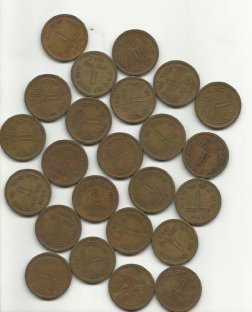
\includegraphics[width = 7cm]{watercoins.jpg}
	\caption{Input image}
\end{figure}



2) Now, we threshold this image
\begin{verbatim}
ret, thresh = cv2.threshold(gray,0,255,cv2.THRESH_BINARY_INV 
                                                    +cv2.THRESH_OTSU)   
cv2.imshow("Otsu", thresh)
\end{verbatim}
\begin{figure}[h]
	\centering
	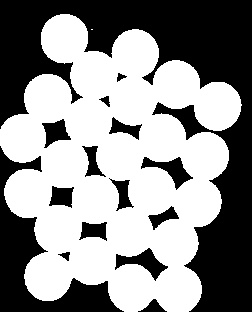
\includegraphics[width = 7cm]{otsuthresh.jpg}
	\caption{Otsu Threshold}
\end{figure}


\newpage
3) To remove noises from the image we use morphological operations. To remove small noises we use opening. To obtain the sure background we dilate the region of the coins and then the result will be the region where we are sure that they don’t contain coins.
\begin{verbatim}
 kernel = np.ones((3,3),np.uint8)
 opening = cv2.morphologyEx(thresh,cv2.MORPH_OPEN,kernel, iterations = 2)
 sure_bg = cv2.dilate(opening,kernel,iterations=3)
\end{verbatim}
\begin{figure}[h]
	\centering
	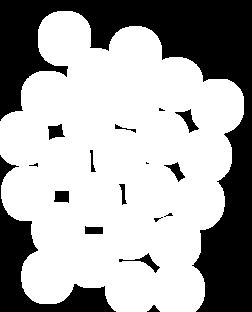
\includegraphics[width = 7cm]{Surebg.jpg}
	\caption{Sure Background}
\end{figure}
%\lstinputlisting[language=Python]{watershed.py}
\newpage
4) Now we have to find the sure foreground region. For this we apply distance transform.
\begin{verbatim}
dist_transform = cv2.distanceTransform(opening,cv2.cv.CV_DIST_L2,5)
ret, sure_fg = cv2.threshold(dist_transform,0.7*dist_transform.max(),
                                                                  255,0)
\end{verbatim}
\begin{figure}[h]
	\centering
	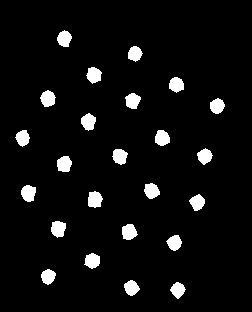
\includegraphics{Surefg.jpg}
	\caption{Sure foreground}
\end{figure} 
\pagebreak
5) The remaining regions are those which we don’t have any idea, whether it is coins or background. Watershed algorithm should find it. These areas are normally around the boundaries of coins where foreground and background meet (Or even two different coins meet). We call it border. It can be obtained from subtracting sure\_fg area from sure\_bg area.
\begin{verbatim}
unknown = cv2.subtract(sure_bg,sure_fg)
\end{verbatim}
\begin{figure}[h]
	\centering
	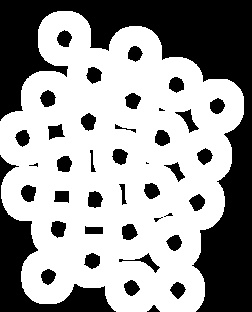
\includegraphics[width = 7cm]{unknown.jpg}
	\caption{Intersection region}
\end{figure}

6) Now we have to create the markers. But before this we have to note that a marker is same size as that of a image but of int32 data type. We will be using sure\_fg image for the marker.
\begin{verbatim}
sure_fg = np.uint8(sure_fg)
\end{verbatim}

7) Now we know for sure which are region of coins, which are background and all. So we create markers and label the regions inside it. The regions we know for sure (whether foreground or background) are labelled with any positive integers, but different integers, and the area we don’t know for sure are just left as zero. Now to do this there are two ways:
\begin{itemize}
	\item For those using python version 3.0 and above :
	\begin{verbatim}
	ret, markers = cv2.connectedComponents(sure_fg)
	markers = markers + 1
	markers[unknown==255] = 0
	\end{verbatim}
	\item For those using python version below 3.0:
	\begin{verbatim}
	contours, hierarchy = cv2.findContours(sure_fg,cv2.RETR_TREE,
	                                            cv2.CHAIN_APPROX_SIMPLE)
	
	#Creating a numpy array for markers and converting the image
	# to 32 bit using dtype paramter
	marker = np.zeros((gray.shape[0], gray.shape[1]),dtype = np.int32)
	
	marker = np.int32(sure_fg) + np.int32(sure_bg)
	
	for id in range(len(contours)):
	cv2.drawContours(marker,contours,id,id+2, -1)
	
	marker = marker + 1
	marker[unknown==255] = 0
	\end{verbatim}
\end{itemize}
\begin{verbatim}
unknown = cv2.subtract(sure_bg,sure_fg)
\end{verbatim}

8) Applying water shed segmentation on the image.
\begin{verbatim}
	   cv2.watershed(img, marker)
	   img[marker==-1]=(0,0,255) # to draw the contours in red 
\end{verbatim}
\begin{figure}[h]
	\centering
	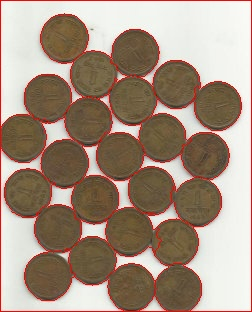
\includegraphics[width = 7cm]{img.jpg}
	\caption{Post watershed image}
\end{figure}

\newpage
9)To observe the image in a colormap we use the matplotlib library.
\begin{verbatim}
  imgplt = plt.imshow(marker)
  plt.colorbar()
  plt.show()
\end{verbatim}
\begin{figure}[h]
	\centering
	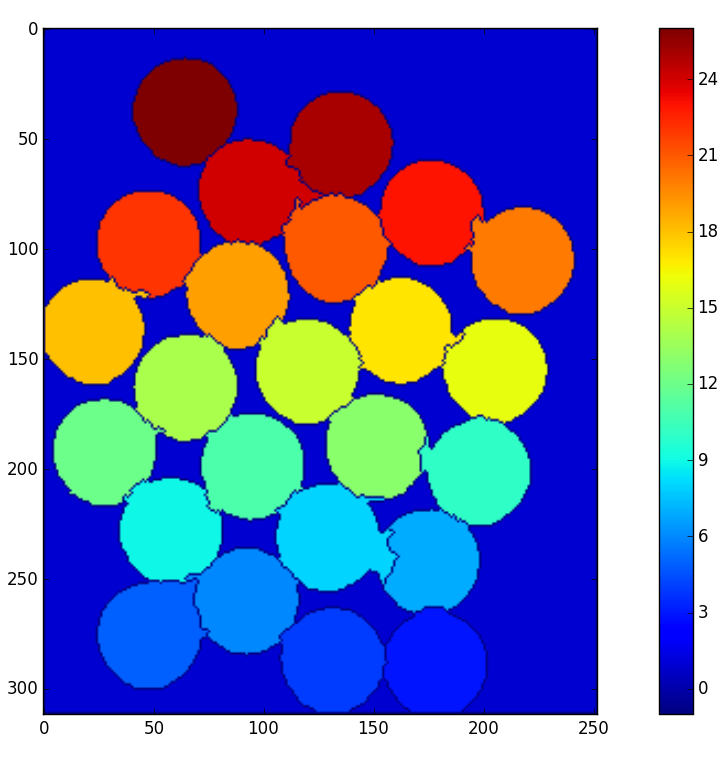
\includegraphics[width = 10cm]{colormap.png}
	\caption{Post watershed image}
\end{figure}

\begin{verbatim}
#import opencvn numpy and matplotlib
import numpy as np               
import cv2
from matplotlib import pyplot as plt

#Reading the image
img = cv2.imread('water_coins.jpg')
gray = cv2.cvtColor(img,cv2.COLOR_BGR2GRAY)        #Conversion to gray scale
ret, thresh = cv2.threshold(gray,0,255,cv2.THRESH_BINARY_INV+cv2.THRESH_OTSU)   #thresholding

cv2.imshow("Otsu", thresh)

# noise removal
kernel = np.ones((3,3),np.uint8)
opening = cv2.morphologyEx(thresh,cv2.MORPH_OPEN,kernel, iterations = 2)

# sure background area
sure_bg = cv2.dilate(opening,kernel,iterations=3)


# Finding sure foreground area
dist_transform = cv2.distanceTransform(opening,
                                        cv2.cv.CV_DIST_L2,5)
ret, sure_fg = cv2.threshold(dist_transform,
                               0.7*dist_transform.max(),255,0)

# Finding unknown region
sure_fg = np.uint8(sure_fg)
unknown = cv2.subtract(sure_bg,sure_fg)

cv2.imshow("Sure bg", sure_bg)
cv2.imshow("Sure fg",sure_fg)
cv2.imshow("unknown",unknown)

#Marker Labelling (for those with python version below 3.0)
contours, hierarchy = cv2.findContours(sure_fg,cv2.RETR_TREE
                                           ,cv2.CHAIN_APPROX_SIMPLE)

# Creating a numpy array for markers and converting the image to 
# 32 bit using dtype paramter
marker = np.zeros((gray.shape[0], gray.shape[1]),dtype = np.int32)

marker = np.int32(sure_fg) + np.int32(sure_bg)

for id in range(len(contours)):
cv2.drawContours(marker,contours,id,id+2, -1)

marker = marker + 1
marker[unknown==255] = 0

"""
# Marker labelling (For those with python version 3.0 and above)
ret, markers = cv2.connectedComponents(sure_fg)

# Add one to all labels so that sure background is not 0, but 1
markers = markers+1

# Now, mark the region of unknown with zero
markers[unknown==255] = 0
"""

cv2.watershed(img, marker)
img[marker==-1]=(0,0,255)

cv2.imshow('watershed', img)

#To display using colormap
imgplt = plt.imshow(marker)
plt.colorbar()               #Creates a bar of colors
plt.show()                   #Displays the windows

cv2.waitKey(0)
cv2.destroyAllWindows()       #Destroys all windows

\end{verbatim}





\newpage
\section{Additional Resources}\label{additional-resources}

\begin{enumerate}
\def\labelenumi{\arabic{enumi})}
\tightlist
\item \href{https://github.com/eyantrainternship/eYSIP_2015_Marker_based_Robot_Localisation/blob/master/Task-2/Watershed%20Segmentation/src/watershed.py}{Code - Github link}
\item \url{http://cmm.ensmp.fr/~beucher/wtshed.html\#examples}
\item \href{http://opencv-python-tutroals.readthedocs.org/en/latest/py
\_tutorials/py\_imgproc/py\_watershed/py\_watershed.html\#watershed}{About watershed segmentation}
\item \href{https://www.cs.auckland.ac.nz/courses/compsci773s1c/lectures
/ImageProcessing-html/topic3.htm}{Image processing lectures}
\item \href{http://stackoverflow.com/questions/11294859 \\ /how-to-define-the-markers-for-watershed-in-opencv}{Info on defining markers}
\end{enumerate}



\end{document}
